\documentclass[8pt]{beamer}
%epackage[french]{babel}
\usepackage[latin1]{inputenc}
\usepackage{listings}
\usepackage{times}
\usepackage{wasysym}
\usepackage[T1]{fontenc}

\usepackage{listings}

\definecolor{mongris}{gray}{0.8}           % definition couleur grise
\newcommand{\dd}{\footnotesize $\Diamond$}

\newcommand{\HH}{ \vspace{0.5pt}\hrule}
\newcommand{\round}[1]{\lceil #1 \rfloor}  % notation arrondi
\def\eme{$^{\textrm{{\`e}me}}$}                  % i {\`e}me
\def\num{n^{\circ}}                        % numero
\def\Num{N^{\circ}}                        % Numero
\def\sinc{\mathrm{sinc}}                   % sinus cardinal
\def\ere{$^{\textrm{{\`e}re}}$}                % {\`e}re
\def\er{$^{\textrm{{e}r}}$}                % {\`e}re
\def\eg{\emph{e.g.} }                      % e.g.
\def\ie{\emph{i.e.} }                      % i.e.
\def\etc{\emph{etc}}                       % etc
\def\cm{\,cm}                              % cm
\def\met{\,m}                              % m
\def\mm{\,mm}                              % mm
\def\deg{$^\circ$}                         % degres
\def\ud{\mathrm{d}}                        % pour dx dy ...


\def \R {{\Bbb R}}
\def \I {{\Bbb I}}
\def \H{{\Bbb H}}
\def \F {{\Bbb F}}
\def \S {{\Bbb S}}
\def \B {{\Bbb B}}
\def \Z {{\mathbb Z}}
\def \G {{\mathbb G}}
\def \L {{\mathcal{L}}}
\def \C {{\mathcal C}}
\def \P {{\mathcal P}}
\def \Q {{\mathcal Q}} 
\def \E{{\mathcal E}}
\def \D{{\mathcal D}}
\definecolor{mybluecolor}{RGB}{116,121,149}

\newcommand{\darky}[1]{{\usebeamercolor[fg]{block title example} #1}}
\newcommand{\myblue}[1]{{\color{mybluecolor}\aut{[#1]}}}

\newcommand{\ball}  {\ensuremath{B}}
\newcommand{\AMDR}{\operatorname{AMD}}
\newcommand{\AMD}{\operatorname{AMD}}

\newcommand{\MAset}{\ensuremath{\mathrm{A\!M}} }
\newcommand{\MAsetg}{\ensuremath{\MAset^g } }

\def \PS {{\aut{Planar-4-3-SAT}}}
\def \R {{\Bbb R}}
\def \I {{\Bbb I}}
\def \F {{\Bbb F}}
\def \S {{\Bbb S}}
\def \Z {{\mathbb Z}}
\def \L {{\mathcal{L}}}
\def \C {{\mathcal C}}
\def \P {{\mathcal P}}
\def \Q {{\mathcal Q}} 
\def \E{{\mathcal E}}
\def \D{{\mathcal D}}
\def \BD {{\bar{\mathcal{D}}}}
\def \etal {{\it et al.~}}
\def\arc{\mbox{arc}}
\definecolor{mongris}{gray}{0.8}          
\newcommand{\fup}[1]{\uparrow#1\uparrow}
\newcommand{\fdown}[1]{\downarrow#1\downarrow}
\newcommand{\sI}[1]{\overline{\tt #1}}
\newcommand{\iI}[1]{\underline{\tt #1}}
\newcommand{\e}[5]{#1 & #2 & #3 & #4 & #5 \\}
\newcommand{\eh}[5]{\text{#1} & \text{#2} &  \text{#3} &  \text{#4} & \text{#5}\\} 

\usepackage{beamerthemeliris2}
\useoutertheme{smoothbars}

\title[Workgroup Digital Geometry]{Introduction to
  DGtal}
\subtitle{\url{http://liris.cnrs.fr/dgtal}}

\author{~}
%\author[DGtal~~~~~~~~~~~~~~~~~~~~~~~~~~David Coeurjolly]{David Coeurjolly}


 \newcommand{\fod}[2]{\multicolumn{2}{p{3.5cm}}{\emph{#1}\dotfill} &
      \multicolumn{2}{p{9cm}}{#2}\\}
    \newcommand{\fodt}[4]{\emph{#1} & {\footnotesize \textsl{#2}} & #3 & \small #4\\}
    % \newenvironment{ta}{\begin{tabular}{p{3.5cm}p{9cm}}}{\end{tabular}\\}
    \newenvironment{ta}{\begin{tabular}{crll}}{\end{tabular}\\}
    % \vfill


\newcommand{\aut}[1]{{\sc #1}}             % auteur en small capsu


%\institute%[XXX]
%{%
%
%  {\bf Laboratoire d'InfoRmatique en Image et Systèmes d'information} \\
%  { \scriptsize{
%  LIRIS UMR 5205 CNRS/INSA de Lyon/Université Claude Bernard Lyon 1/Université Lumiè%re Lyon 2/Ecole Centrale de Lyon\\
%  INSA de Lyon, bâtiment J. Verne\\
%  20, Avenue Albert Einstein - 69622 Villeurbanne cedex\\
%  \url{http://liris.cnrs.fr}}
%  }
%}



\graphicspath{{./Figures/}, {./../images/},{./Fig/}, {./ICPR2010/},{./Antoine/images/}; {./Images/}}


\begin{document}

\small






\begin{frame}[plain]
  \titlepage
\end{frame}

%------------------------------------------------------------------------------
\begin{frame}%[allowframebreaks]
  \frametitle{DGtal: why, who}
  
  \small
  \begin{block}{Objectives}
    \small
    \begin{itemize}
    \item to make digital geometry easier for the neophyte (student,
      researcher from another field, \ldots)
    \item to test quickly new ideas, with objective comparison wrt
      existing works
    \item to make easier the implementation of demonstrators
    \item to help spread our research results to other domains
    \end{itemize}
  \end{block}
  
\alert{$\Rightarrow$ Federative Project}
  
  \small
  \begin{block}{Who ? for now \ldots}
    \small
    \begin{columns}
      \begin{column}{0.45\textwidth}
        \begin{itemize}
        \item LIRIS (Lyon)      
        \item Gipsa-lab (Grenoble)
        \item GREYC (Caen)
        \end{itemize}
      \end{column}
      \begin{column}{0.45\textwidth}
        \begin{itemize}
        \item LAMA (Chamb�ry)
        \item LORIA (Nancy)
        \item IRCCyn (Nantes)
        \end{itemize}
      \end{column}
    \end{columns}
  \end{block}
\end{frame}
%------------------------------------------------------------------------------

%------------------------------------------------------------------------------
\begin{frame}%[allowframebreaks]
  \frametitle{DGtal: what for ?}
  
  \small
  \begin{block}{Main features}
    \small
    \begin{itemize}
    \item to define digital objects in arbitrary dimension
    \item to propose algorithms for topological and geometric analysis
    \item to provide I/O mechanisms and visualization tools
    \end{itemize}
  \end{block}
  \medskip

 \hspace*{-1cm} \begin{tabular}{ccccc}
    \includegraphics[height=0.1\textheight]{exampleDSS-3}
    &
    \includegraphics[height=0.15\textheight]{edt-2d}
    &
    \includegraphics[height=0.15\textheight]{object-3d-18-6}
    &
    \includegraphics[height=0.15\textwidth]{thinning-3d}
    &
    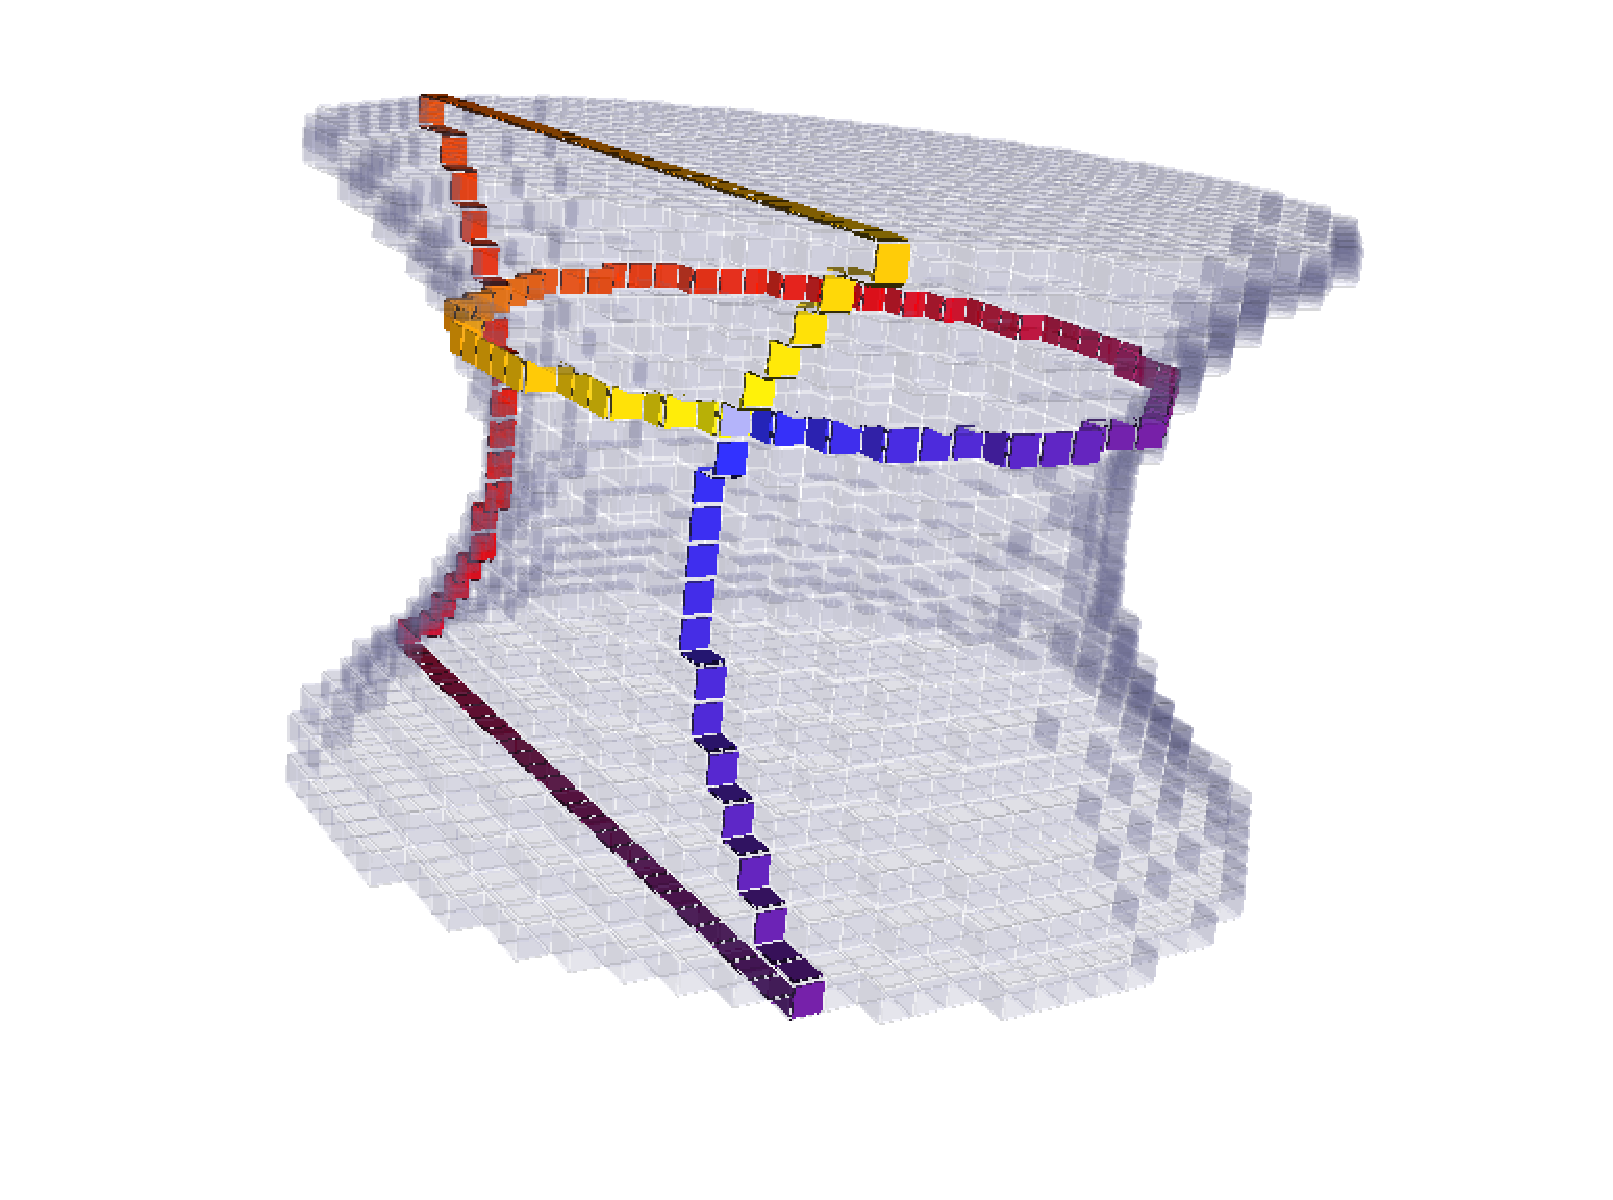
\includegraphics[height=0.15\textwidth]{surfelTracking}
    \\
    DSS & DT & Objects & Thinning & Cellular model\\
    \includegraphics[height=0.2\textheight]{lengths-ball-R10-bis}
    &
    \includegraphics[height=0.15\textheight]{shapes}
    &
    \includegraphics[height=0.15\textwidth]{klokanNoise}
    &
    \ldots
    &
    %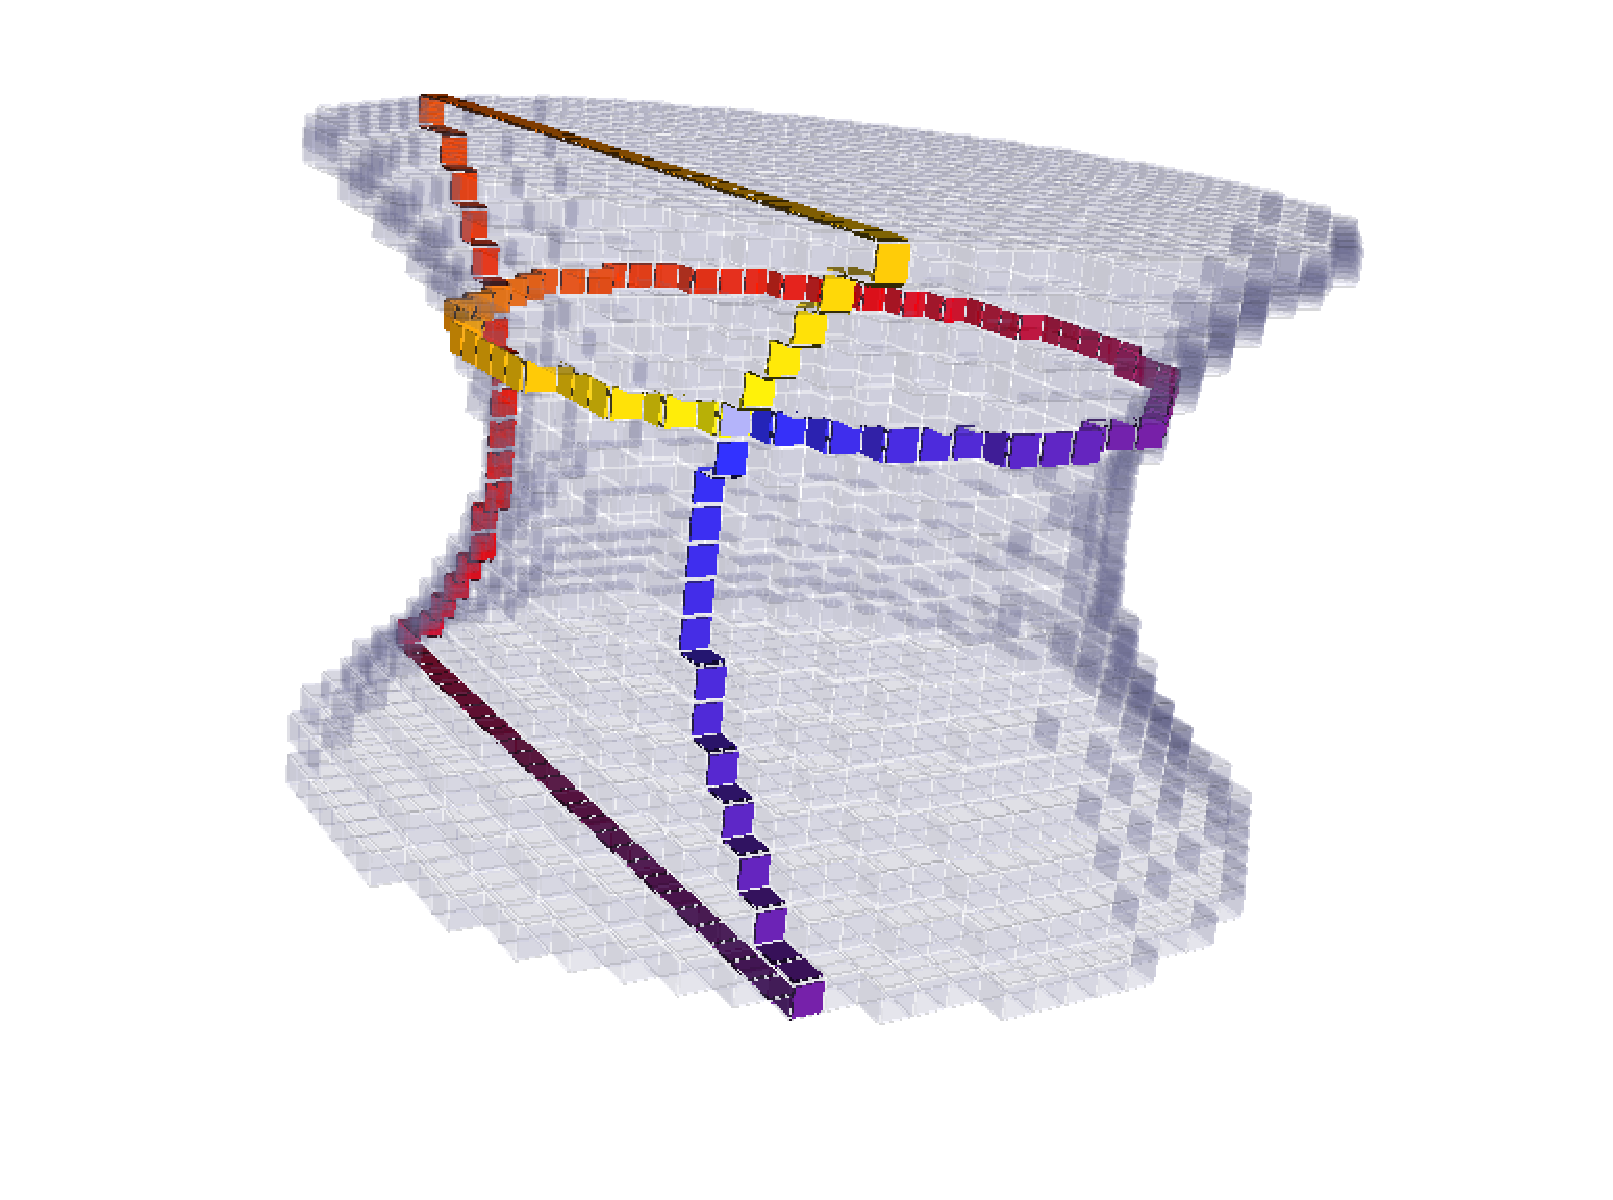
\includegraphics[height=0.15\textwidth]{surfelTracking}
    \\
    Estimators & Shape DB& Contours & 
  \end{tabular}

\end{frame}
%------------------------------------------------------------------------------
%------------------------------------------------------------------------------
\begin{frame}%[allowframebreaks]
  \frametitle{DGtal philosophy and structure}

  \begin{block}{}
    \small
    \begin{itemize}
    \item  Genericity and efficiency: C++ library, concepts
    \item  LGPL
    \item Cmake build system (linux/macOS/MSwindows)
    \item user friendly, not necessarily kernel-developer friendly
    \end{itemize}
  \end{block} 
  \begin{alertblock}{\centering Kernel Package\HH}
    \begin{columns}
      \begin{column}{0.44\textwidth}
        \begin{alertblock}{Basic types, data structures}
          \small
          \begin{itemize}
          \item Digital space
          \item  Point, vectors
            \item Digital domains and digital sets
             \item  \ldots  
          \end{itemize}
        \end{alertblock}
      \end{column}
      \begin{column}{0.44\textwidth}
        \begin{alertblock}{Arithmetics \& Linear Algebra}
          \footnotesize
          \begin{itemize}
          \item Integer, BigInteger (arbitrary precision)
          \item Number traits
          \item Basic linear algebra
          \item \ldots
          \end{itemize}
        \end{alertblock}
      \end{column}
    \end{columns}
  \end{alertblock}
  \begin{alertblock}{\centering Topology Package\HH}
    \small
       \begin{itemize}
    \item Digital Topology: connectedness, border, simple points
      (\emph{a la} Rosenfeld)
    \item Cartesian Cellular Topology: cells,  surfaces and contours
      (\emph{a la} Herman), tracking algorithms
    \end{itemize}
  \end{alertblock}
\end{frame}

\begin{frame}
  \frametitle{DGtal philosophy and structure}
    \begin{alertblock}{\centering Geometry Package\HH}
    \small
    \begin{itemize}
    \item Primitives: DSS recognition
    \item Contour analysis: decomposition, convexity, estimators
    \item Volumetric analysis: area/volume, distance transforms,
      reverse distance transforms
    \item Implicit/parametric shape generator for multigrid analysis
    \end{itemize}
  \end{alertblock}
  
  \begin{alertblock}{\centering Image Package\HH}
    Image concept and Image containers, e.g.
    \begin{itemize}
    \item Image by STL \texttt{vector} (linearized nD image)
    \item Image by STL \texttt{map} (mapping points$\leftrightarrow$values)
    \item HashTree image container (generalized octree with hashing functions)
    \end{itemize}
  \end{alertblock}
  

  \begin{alertblock}{\centering IO Package\HH}
    \small
    \begin{itemize}
    \item \texttt{Boards}: export to illustrate objects/algorithms (eps,pdf,svg,png,tikz\ldots)  
    \item \texttt{Viewers}:  simple 3D viewer (Qt/QGlViewer)
    \item Readers/writers for various image formats
    \end{itemize}
  \end{alertblock}
\end{frame}
%------------------------------------------------------------------------------
%------------------------------------------------------------------------------
\begin{frame}%[allowframebreaks]
  \frametitle{DGtal}
\small
  \begin{block}{ New in milestone 0.4}
    \small
    \begin{description}
        \item[Global changes] decomposition of DGtal algorithms and
        data structures into packages, concepts and concept checking mechanism have been
        considerably improved.
      \item[Kernel Package] refactoring of Integer types considered in DGtal.
       \item[Topology Package] Interpixel/cellular topological models, boundary tracking tools,...
       \item[Geometry Package] multi-modal representation of 1D
         contours and curves (GridCurve facade), decomposition/segmentation into primitives,
        many differential estimators added...
       \item [I/O Package] refactoring/enhancements of DGtal boards and viewers, enhancement of 2D boards with libcairo and a new Board3Dto2D board has been added.
       \item [Tools] multigrid shapeGenerator/contourGenerator added, lengthEstimator/estimatorComparator added for differential estimator multigrid comparison, connected components extraction in 3D,...
       \item [Documentation] User guide has been improved thanks to a decomposition of the library into packages.
\end{description}
  \end{block}

  %% \begin{alertblock}{Join DGtal}
  %%   \small
  %%   \begin{itemize}
  %%   \item new contributors are welcome (new bug-reporters, documentation readers are welcome too)
  %%   \item collaborative forge, development infrastructure
  %%   \end{itemize}
  %% \end{alertblock}
  
\end{frame}



\lstset{ language=[Visual]C++,
	keywordstyle=\bfseries\ttfamily\color[rgb]{0,0,1},
	identifierstyle=\ttfamily,
	commentstyle=\color[rgb]{0.133,0.645,0.133}\textit,
	stringstyle=\ttfamily\color[rgb]{0.627,0.126,0.941},
	showstringspaces=false,
	basicstyle=\ttfamily,
	numberstyle=\color[rgb]{0.2,0.2,0.2}\tiny\ttfamily,
	numbers=left,
	stepnumber=1,
        frame=single,
        framexleftmargin=13mm, 
        xleftmargin=12mm,
	numbersep=10pt,
	tabsize=2,
	breaklines=true,
	prebreak = \raisebox{0ex}[0ex][0ex]{\ensuremath{\hookleftarrow}},
	breakatwhitespace=false,
	aboveskip={1.5\baselineskip},
  columns=fixed,
  upquote=true,
  extendedchars=true
}

\begin{frame}[containsverbatim]
\frametitle{DGtal program skeleton}

  \begin{lstlisting}
    
    #include "DGtal/base/Common.h"
    #include "DGtal/kernel/SpaceND.h"
    #include "DGtal/kernel/domains/HyperRectDomain.h"
    ...
    typedef DGtal::int32_t Integer;
    typedef DGtal::SpaceND<4, Integer> Space;
    typedef Space4::Point Point;
    typedef HyperRectDomain<Space> Domain;
    
    Point p(12, -34,0,1);
    Point q(2, -2, -1,3);
    if (p < q)
    ...
    
    Domain box(p,q);
    ....

  \end{lstlisting}
\end{frame}

%------------------------------------------------------------------------------
%------------------------------------------------------------------------------
\begin{frame}
  \frametitle{DGtal Team}

   \begin{center}
     \includegraphics[width=0.3\textwidth]{dgtal-logo}\\
     \url{http://dgtal.org}
 ~\\
    \url{http://github.com/DGtal-team}
  \end{center}

   %%       \begin{tikzpicture}[remember picture,overlay]
   %%         \input{lama.logo}
   %%       \end{tikzpicture}
   \begin{center}
     \small
     \includegraphics[width=1.5cm]{liris-logo}
     \quad
     \includegraphics[width=1.5cm]{lama-logo}
     \quad
     \includegraphics[width=1.5cm]{loria-logo_new}
     \quad
     \includegraphics[width=1.5cm]{greyc-logo}
     \quad
     \includegraphics[width=1.5cm]{gipsa-logo}
     \quad
     \includegraphics[width=1.5cm]{irccyn_transparent}
   \end{center}
 \small

\begin{center}
  David Coeurjolly <david.coeurjolly@liris.cnrs.fr>,
  Jacques-Olivier Lachaud <jacques-olivier.lachaud@univ-savoie.fr>,
  Bertrand Kerautret <kerautre@loria.fr>,
  Tristan Roussillon <tristan.roussillon@liris.cnrs.fr>,
  Isabelle Sivignon <isabelle.sivignon@gipsa-lab.grenoble-inp.fr>,
  Guillaume Damiand <guillaume.damiand@liris.cnrs.fr>,
  Sebastien Fourey <Sebastien.Fourey@greyc.ensicaen.fr>,
  Martial Tola <martial.tola@liris.cnrs.fr>,
  Xavier Proven�al <xavier.provencal@univ-savoie.fr>,
  Aline Martin <aline.martin@insa-lyon.fr>,
  Pierre Gueth <pierre.gueth@liris.cnrs.fr>,
  Adrien Kr�henb�hl <adrien.krahenbuhl@loria.fr>,
  Anis Benyoub <anis.benyoub@liris.cnrs.fr>,
  Nicolas Silva <nicolas.silva@insa-lyon.fr>,
  J�r�my Gaillard <jeremy.gaillard@insa-lyon.fr>,
  J�r�my Levallois <jeremy.levallois@liris.cnrs.fr>
\end{center}

\end{frame}
%------------------------------------------------------------------------------

%-%% -----------------------------------------------------------------------------

%% %------------------------------------------------------------------------------


\begin{frame}
  \frametitle{DGtal's Future}
  
  \begin{block}{ToDo List}
    \begin{description}
    \item [Kernel] Enhance the Linear Algebra module (more operations,\ldots )
    \item [Geometry] implement more estimators on 2D contours and 3D
      surfaces, finish the medial axis backport, implicit/parametric
      shapes in 3D, noise detection and handling
    \item [Topology] add a combinatorial model to handle partitions, 
    \item [IO] enhance bindings with external libs (ITK, VIGRA, Olena,
      ...)
    \item[Image] add out-of-core containers, refactor image \emph{morphers}    
    \end{description}
  \end{block}
  
  
  \begin{exampleblock}{Wishlist}
    \begin{description}
    \item [Mathematical Morphology] either with a binding or with an
      implementation from scratch
    \item [Discrete Tomography] ;)
    \end{description}
  \end{exampleblock}


  \begin{alertblock}{}
    \alert{Users, Bug reporters,  Doc checkers, Developers,...}
  \end{alertblock}

\end{frame}


\end{document}



%Sample.dat -> GRidCurve -> board (GC, GC::Arrows, GC::Inci)

%Image -> Set ->  DT -> board

%Image -> contour (KSpace, track) -> GC -> estimateur (longueur)

%Shape -> Digitizer -> Contour -> GC -> Estimateur

% Shape -> surface -> viewer

% Shape -> Surface -> slice -> GC -> longueur (viewer Segm.DSS)
